% PLEASE USE THIS FILE AS A TEMPLATE
% Check file iosart2c.tex for more examples
%
% Journal:
%   Semantic Web (sw)
% IOS Press
% Latex 2e

% add. options: [seceqn,secfloat,secthm,crcready,onecolumn]

\documentclass[sw]{iosart2c}

\usepackage[numbers]{natbib}% for bibliography sorting/compressing
%\usepackage{amsmath}
%\usepackage{endnotes}

\usepackage{graphicx} % needed for command \includegraphics, also supports width

%%%%%%%%%%% Put your definitions here


%%%%%%%%%%%%%%%%%%%%%%%%%%%%%
% User-defined commands
%%%%%%%%%%%%%%%%%%%%%%%%%%%%%


\usepackage{tabulary}
\usepackage{multirow}
% \usepackage{booktabs} % provides \toprule, \midrule, \bottomrule for table


% \usepackage{geometry}
\usepackage{color}
\usepackage{colortbl} % needed for coloring table, see: https://texblog.org/2011/04/19/highlight-table-rowscolumns-with-color/
\usepackage[table]{xcolor} % needed for coloring table, see: https://en.wikibooks.org/wiki/LaTeX/Tables

%\definecolor{name}{system}{definition}
\definecolor{Gray}{gray}{0.9}
\definecolor{LightCyan}{rgb}{0.88,1,1}




\setlength{\paperheight}{297mm} % needed for package {hyperref}

%\usepackage{hyperref}
\usepackage[draft]{hyperref} % defined as 'draft' to avoid error message http://tex.stackexchange.com/questions/1522/pdfendlink-ended-up-in-different-nesting-level-than-pdfstartlink

\usepackage{url}


%
% TABULARS
%

% This command is to add new lines in tables
% See manual: http://tex.stackexchange.com/questions/2441/how-to-add-a-forced-line-break-inside-a-table-cell

\newcommand{\specialcell}[2][c]{%
  \begin{tabular}[#1]{@{}l@{}}#2\end{tabular}}



%
% LISTINGS
%

\usepackage{listings} % see manual: ftp://ftp.funet.fi/pub/TeX/CTAN/macros/latex/contrib/listings/listings.pdf

%
% Change caption font size: http://tex.stackexchange.com/questions/129291/change-caption-style-of-listings-package-without-caption-package
%
\usepackage[font=bf,skip=\baselineskip]{caption}
\captionsetup[lstlisting]{font={footnotesize,sf}}

% language Ruby is used to enable comment lines started with hash character

\lstset{language=Ruby,
aboveskip=6pt,
belowskip=6pt,
backgroundcolor=\color[gray]{0.85},
numberstyle=\scriptsize,
basicstyle=\linespread{0.9}\ttfamily\scriptsize,
% aboveskip={-4ex},
numbers=none,
stepnumber=1,
frame=none,
breaklines=true,
breakautoindent=true}

\AtBeginDocument{%
  \renewcommand{\thelstlisting}{\arabic{lstlisting}}
 }

%\spnewtheorem{principle}{Principle}{\bfseries}{\rmfamily}

% \AtBeginDocument{
%     \newtheoremstyle{principleStyle}
%         {1.5\topsep} % Space above, default \topsep
%         {0.5\topsep} % Space below, default \topsep
%         {\itshape} % Body font
%         {} % Indent amount, example: \parindent
%         {\bfseries\itshape} % Theorem head font
%         {.} % Punctuation after theorem head
%         {.5em} % Space after theorem head
%         {} % Theorem head spec (can be left empty, meaning `normal')
        
%     \theoremstyle{principleStyle} \newtheorem{principle}{Principle}
% }




% Commands for C#, C++
% Source: https://www.johndcook.com/blog/2011/10/18/typesetting-c-in-latex/
\newcommand{\CPP}{C\nolinebreak\hspace{-.05em}\raisebox{.4ex}{\tiny\bf +}\nolinebreak\hspace{-.10em}\raisebox{.4ex}{\tiny\bf +}}
\newcommand{\CS}{C\nolinebreak\hspace{-.05em}\raisebox{.6ex}{\scriptsize\bf \#}}






%\usepackage{linegoal}

% \newcommand{\definition}[1]{\textbf{#1}}
%\newcommand{\name}[1]{\emph{#1}}

% programming language names
\newcommand{\name}[1]{\textsf{\footnotesize{}#1}}

% highlight texts
%\newcommand{\highlight}[1]{\colorbox{yellow}{\parbox[t]{\linegoal}{#1}}}
\newcommand{\highlight}[1]{\colorbox{yellow}{\parbox[t]{\hsize}{#1}}}


% TODO text
% \newcommand{\TODO}[1]{\highlight{\textbf{TODO: }{#1}}}
\newcommand{\TODO}[1]{{}}

%\newcommand{\REVIEW}[1]{\textit{#1}}

% ifcOWL layer names
\newcommand{\bname}[1]{\textnormal{\textbf{#1}}}

\newcommand{\simple}{\bname{Simple}}
\newcommand{\standard}{\bname{Standard}}
\newcommand{\extended}{\bname{Extended}}

\newcommand{\ifcowl}{\bname{ifc\-OWL}}
\newcommand{\ifcrdf}{\bname{ifc\-RDF}}
\newcommand{\ifcsimple}{\ifcowl{}-\simple{}}
\newcommand{\ifcstandard}{\ifcowl{}-\standard{}}
\newcommand{\ifcextended}{\ifcowl{}-\extended{}}

\newcommand{\ifcconverter}{\bname{IFC2LD}}
\newcommand{\ifcld}{\ifcconverter}


%%%%%%%%%%% End of definitions

\pubyear{2017}
\volume{0}
\firstpage{1}
\lastpage{1}

\begin{document}


% Added to enable emphased text hyphenation
\sloppy



\begin{frontmatter}

%\pretitle{}
%\title{Designing common mechanisms \& tools for conversion of various building data formats into OWL \& RDF}
\title{Conversion of building data formats into OWL \& RDF: Towards common mechanisms \& tools}
% \runningtitle{Designing common mechanisms \& tools for conversion of various building data formats into OWL \& RDF}
\runningtitle{Conversion of building data formats into OWL \& RDF: Towards common mechanisms \& tools}
%\subtitle{}

%\review{}{}{}


% For one author:
\author{\fnms{Nam} \snm{Vu}}
\address{Aalto University, Espoo, Finland\\Email: nam.vuhoang@aalto.fi}
\runningauthor{}

\begin{abstract}
Conversion of building data schemas and sets to OWL ontologies and RDF datasets accordingly is one of the most significant steps to enable Web of Building Data, i.e. sharing and interlinking distributed building information with Web of Data technologies.
So far, building data, including all kinds of information related to the building life cycle, is mainly exchanged in file formats SPF, XML, CSV, and spreadsheets; while their data schemas are specified with EXPRESS or XSD languages.
For instance, IFC (Industry Information Classes) defines an EXPRESS based data model and multiple exchange formats IFC-SPF, IFC-XML, and IFC-ZIP.
In 2015, a group of researchers agreed on the key principles of translating IFC-EXPRESS schema and IFC-SPF datasets into OWL and RDF.
In this paper, I discuss the current IFC-to-RDF conversion mechanism, propose the ways of its optimization, and analyze how to apply similar principles for the XML-based formats, such as COBie, bsDD, InfraXML.
Finally, we introduce our open-source Java conversion software, the central part of which is a dynamic Java entity-relationship model based on both EXPRESS and XSD data models.
By including new plugins, this software allows converting other industrial formats, not only in the built environment. 
 
\end{abstract}

\begin{keyword}
 Web Ontology Language (OWL)
 \sep
 Resource Description Framework (RDF)
 \sep
 Industry Foundation Classes (IFC)
 \sep
 EXPRESS
 \sep
 XSD
 \sep
 XML
 \sep
 STEP Physical File (SPF)
\end{keyword}

\end{frontmatter}

% \section{Introduction}\label{introduction}



Nowadays, in the Architecture, Engineering, Construction and Facility Management (AEC/FM) industry, problems of integrating, accessing and reasoning over \emph{big building-related data}, which is dynamic, interrelated, heterogeneous and fragmented, is crucial.
Throughout the life cycle of a building in modern AEC/FM projects, different parties (people and automatic systems) are involved in producing and utilizing vast volume of information about the building, including both structured and non-structured data.
Our research focuses on the structured building-related data, denoted here for brevity as \emph{building data}.
Building datasets are often developed separately and concurrently, with variable change frequencies depending on their domains and the ongoing life cycle phase.
For instance, during the facility management stage, the 3D architectural model of the building is unchangeable while the sensor data about its indoor environment is updated every few minutes.
Most of the conceptual data schemas and datasets are semantically interrelated (directly or indirectly) because they describe various aspects about the same or similar physical objects, however, they are mainly disintegrated and managed in a fragmented manner.
Moreover, the significant increase in the number of data schemas and serialization formats also made exchanging, integrating or linking data between parties much harder. 
In general, the relevant building data is difficult to access, disconnected from potential users and related systems, and remains underutilized. \cite{torma2012distributed}.





Building Information Modeling (BIM), one of the most notable efforts in recent years regarding AEC/FM information management, can solve only a part of the mentioned problems.
BIM appeared as a new approach "in which a digital representation of the building process is used to facilitate the exchange and interoperability of information" \cite{eastman2011bim} and now turned into a standard process a many countries.
One of major innovations of BIM is the Industry Foundation Classes (IFC) standard, developed by buildingSMART and is currently widely used.
...
....



is a fast developing 



appeared as a new approach to 

aims to facilitate the data exchange and interoperability, 

a new approach for AEC/FM information management \cite{eastman2011bim}, has appeared and quickly turned into a standard process in 

many countries. 
Although in BIM, many native data formats must be translated into a common text format called \emph{Industry Foundation Classes (IFC)} \cite{liebich2016ifc4} 

data exchange, which, however, is still file-based and problematic due to big sizes of datasets. 


even after the rise of Building Information Modeling (BIM), 


Within Building Information Modeling (BIM) \cite{eastman2011bim}, a fast developing standard process for construction information management during the last years, many native data formats are translated into a common text format called \emph{Industry Foundation Classes (IFC)} \cite{liebich2016ifc4} to the facilitate data exchange, which, however, is still file-based and problematic due to big sizes of datasets. 




Linked Building Data, or Web of Building Data, is an emerging trend of using the Semantic Web and Linked Data technologies to address the mentioned data management problems in the AEC/FM industry.
On the one hand, the Semantic Web provides standards and related tools for representing and querying data,
(i) by defining Resource Description Framework (RDF) as a universal data format,
(ii) by specifying schema languages such as Web Ontology Language (OWL) for adding rich semantics to the data,
and (iii) by constructing SPARQL, a standard query language for RDF \cite{polleres2013rdfs}.
Moreover, the Semantic Web offers rule languages, rule-based inferencing engines and other mechanisms for reasoning, i.e. "deriving facts that are not expressed explicitly in machine-readable ontologies or knowledge bases" \cite{sikos2015mastering}.
On the other hand, Linked Data establishes a set of core principles and best practices for publishing structured data on the Web as interlinked RDF graphs.
The core principles are simple: use HTTP URIs to name things, return RDF about those things when their URIs are looked up, and include links to related RDF documents elsewhere on the Web \cite{bizer2009linked, hogan2014linked, polleres2013rdfs}.
By applying simultaneously the Semantic Web standards and the Linked Data principles and best practices, Linked Building Data allows the building data to be effectively deployed on the Web in a manner that facilitates their discovery and interoperability.




One of the first major steps to enable Linked Building Data is conversion of IFC data models and data into OWL ontologies and RDF datasets correspondingly.
The IFC data model is a platform neutral and open file format specification, commonly used collaboration format in BIM.
The conceptual data schema of IFC, developed by buildingSMART, is object-based and can be specified either in \emph{EXPRESS}, a standard data modeling language for product data, or in the W3C XML Schema Definition language (XSD).
EXPRESS is defined in ISO 10303, which is informally known as \emph{"STEP"} (Standard for the Exchange of Product model data).
IFC data in turn can be serialized in different file formats, namely IFC-SPF, IFC-XML, or IFC-ZIP.
IFC-SPF and IFC-XML are based on two STEP text formats, called \emph{STEP-file} (or \emph{STEP Physical File}) and \emph{STEP-XML} accordingly. 
IFC-ZIP is a ZIP compressed format consisting of an embedded IFC-SPF.
All BIM tools, such as Revit, ArchiCAD or Tekla, in addition to their native data formats, must be able to produce and utilize one or more IFC data formats.
In order to be used in Linked Building Data, according to the Semantic Web and Linked Data principles, the IFC data schemas (there are several versions) must be converted into OWL ontologies (RDFS is not used because it provides poor semantics and it is included in OWL profiles), and IFC data files must be translated into RDF datasets consistent with the OWL ontologies.




In 2015, a set of guidelines for the IFC-EXPRESS-to-OWL and IFC-SPF-to-RDF conversion processes was established, and later one of the resulting \emph{ifcOWL} ontology variations was assigned by buildingSMART a bSI Candidate Standard status, despite certain disadvantages.
At the 3rd Linked Data in Architecture and Construction Workshop (LDAC2015), different approaches of the IFC-to-RDF conversion, presented in \cite{pauwels2016express, vu2015implementation, vu2014opening}, were compared and merged in order to form conversion guidelines for generating the only \emph{one} ifcOWL ontology for each IFC data schema version (aka. IFC specification)\cite{pauwels2015third}.
This ontology must contain \emph{all} possible data type restrictions that describe the original IFC data schema and are allowed in OWL 2 DL, one of the most powerful profiles of the OWL 2 Web Ontology Language (informally OWL 2) in term of expressiveness.
As pointed out in \cite{pauwels2016express}, "the disadvantage behind this decision is that the resulting ifcOWL ontology will imply sacrifices in terms of performance, in particular reasoning performance".
Moreover, in spite of semantic richness of OWL 2 DL, data type restrictions in OWL are rarely and hardly used for data validation due to the Open World Assumption (OWA), mainly used in the Semantic Web, opposite to traditional programming environments which prefer the Closed World Assumption (CWA), according to which what is not known to be \texttt{true}, must be considered as \texttt{false}.
Unfortunately, the compliance with the Linked Data principles and some other issues were also not taken into account when making the conversion guidelines.
Therefore, produced \emph{ifcRDF} datasets may be unpublishable in Linked Data or useless in terms of linking with other datasets, for instance, if they contain blank nodes, i.e. resources without URIs, or unstable URIs, which refer to different "things" in distinct versions.
Nevertheless, the resulted ifcOWL ontology of one of IFC-EXPRESS-to-OWL converters, which was made by P.Pauwels and W.Terkaj \cite{pauwels2016express} according to the conversion guidelines, was approved as a bSI Candidate Standard and is currently used as a recommended version in the W3C Linked Building Data (W3C-LBD) community.





Practice shows that the multilayering ontology approach proposed and implemented by us in \cite{vu2015implementation} and also presented at LDAC2015 is more rational.
This approach, compared to the case with an all-in-one ifcOWL ontology as the only ontology, facilitates more real-world scenarios, from querying and reasoning with Semantic Web technologies to publishing and linking datasets with Linked Data technologies.
The key idea is to generate:
(i) \emph{several} {ifcOWL} variations for each IFC data schema version, so that users can switch between different OWL 2 profiles when needed;
and (ii) in the same time only \emph{one} {ifcRDF} dataset for each IFC data file.
These {ifcOWL} variations are subsets of each other and named as layers.
The \emph{ifcOWL-Simple}, \emph{ifcOWL-Standard}, and \emph{ifcOWL-Extended} layers are compatible with the OWL 2 EL, OWL 2 RL, and OWL 2 DL profiles accordingly; where ...
% the lightweight OWL 2 EL profile, more complex OWL 2 RL profile, and OWL 2 DL, the most complicated profile after OWL 2 Full.
The user choice of an ifcOWL layer depends on the task requirements and the tools used because different reasoners support different OWL profiles \cite{w3c2017owlimplementations, manchester2017reasoners}, while simple querying with SPARQL or linking datasets throught URIs do not require any ontology.
On the one hand, the requirement of ....
Certainly, the only ifcRDF dataset for each IFC data file must be compatible with all ifcOWL layers and, consequently, all OWL 2 profiles in which they belong.
This requirement ensures that the ifcRDF dataset can be used for all tasks without re-conversion, but it also involves certain restrictions.
In particular, the use of datatypes \texttt{xsd:double}, \texttt{xsd:boolean} and anonymous individuals (blank nodes) must be avoided, because they are not allowed in OWL 2 EL.
To ensure flexibility, our dual IFC-EXPRESS-to-OWL and IFC-SPF-to-RDF converter supports configuration options, to enable the users, in case they know exactly the application scope of the ifcRDF datasets, to force the converter not naming every object with an URI.
This converter has been tested successfully in many proof-of-concept projects of Linked Building Data with different objectives: from information extraction to linking data.




In addition to IFC-EXPRESS data schemas and IFC-SPF data files, there are many data formats used in the AEC/FM insdustry, which can be divided into five different categories, which, however, have similar properties.

% SPF, XML, CSV, Spreadsheets, and relational databases.








% % OWL 2 DL is a profile of the OWL 2 Web Ontology Language (informally OWL 2), which supports so called Description Logic (DL) and is a superset of other profiles, namely OWL 2 EL, OWL 2 QL, and OWL 2 RL (see Figure 1).
% % None of these profiles can construe very specific EXPRESS language terms such as functions, derived attributes and rules.
% % Thus, the main focus was to build an \emph{all-in-one} ontology using the full expressive power of OWL 2 DL, ignoring the computational complexity it involves.
% % Moreover, 


% , which can be considered as guidelines,







% % However, typical reasoning tasks over ontologies described in the unrestricted OWL (2) Full language are undecidable, i.e. they cannot be guaranteed to ever terminate \cite{hogan2014linked, motik2009owl}.
% Last but not least, the guideline was incomplete and left many issues open. 
% The decision to remain in OWL 2 DL, 

% In spite of this and other drawbacks, pointed in Chapter 2.2, the result ifcOWL ontology was later accepted by buildingSMART as a Candidate Standard and .







% Only IFC-EXPRESS data schemas and IFC-SPF files, which are most widely used in BIM, were taken into account as the inputs of the conversion.
% As result, the formed a fundamental conversion guideline 

% convert only particular data formats and to 


% Practice shows that some solutions proposed by us in ... and presented but was not taken into account seriously in LDAC2015 



% % In general, the agreed principle list do not solve 
% % leave many open questions such as whether to use super properties in so called Drummond 
% % As result, 





% % The practice shows that many the ideas 








% % In 2015, the Linked Building Data community made some agreements 



% % By default, an IFC data file is converted to one separate ifcRDF dataset.






% % building data, especially IFC models, into RDF.  



% % ...  is Linked Building Data (LBD)

% % The main data formats in BIM are:

% % The main challenges/requirements are

% % One of the first steps to enable Linked Building Data is converting different kinds of data schemas and datasets into OWL ontologies and RDF datasets. IFC, EXPRESS, XSD, XML.

% % In 2015, the LBD community IFC-to-RDF .... was accepted as buildingSMART adaf 
% % LDAC 2015, Because the main focus was to provide an ontology: which is (a) describes as much. Therefor, many proposals from [] were ignored by the community:... Moreover, many issues remained open: blank nodes, adfadfadf 

% % This violates recommendations of (W3C), (Aidan Hogan): ....

% % The practical real-world scenario also showed....

% % In this paper, (chapter by chapter) 

% % In Chapter 2, we redefine the requirements...., analyze the problems of OWL, ...










% % ; however, the using the Web-of-Data technologies can solve many of them.
% % Over the lifecycle of a building, different parties involved produce and utilize more and more data.
% % Unfortunately, these building-related data have different formats, are fragmented into separate information silos, and are difficult to link on both logical and physical levels. The authors in (Beetz 2009a, Beetz et al 2009b, Pauwels et al 2011, Törmä 2013, Törmä 2014) proposed to use the Web-of-Data technologies, i.e., the combination of Semantic Web and Linked Data, to address the problems. Today this approach is getting very popular, since it gives significant potential benefits:
% % •	the data about individual building objects could be accessed in a granular fashion;
% % •	the online access brings the same, most recent version of the data available for all parties;
% % •	data management can be distributed according to the structure of any project consortium;
% % •	the semantic description of data enables the automation of workflows and reasoning tasks;
% % •	and possibilities of cross-dataset linking allow the integration of data from multiple datasets based on the needs of use cases.



% % \TODO{(Conclusion sentence?)}

 




% % \highlight{
% %  - SPF (Standard for the exchange of product model data Physical File)\\
% %  - At the 3rd International Workshop on Linked Data in Architecture and Construction (LDAC 2015), the researchers \\
% %  -  based on our theoretical analysis and practical use\\
% %  - whether it is possible and how to...\\
% %  - IFC is is commonly used collaboration format in Building Information Modeling (BIM) based projects, 
% %  - the Java object model allows to represent almost all kind of object-oriented data used in industry and then convert them to RDF with minimum possible loses. Therefore ...\\
% % - enough to write a plugin to convert data then convert\\
% % - this tool can be also used for any other industrial object-oriented data formats, not only in the Built Environment. \\
% % - COBie (Construction Operations Building Information Exchange), bsDD (buildingSMART Data Dictionary), \\
% % - IFC-ZIP (compressed IFC-SPF)\\
% % - The buildingSMART community accepts the generated ifcOWL ontologies as Candidate Standards.\\
% % - the software can be used stand-alone or as part of other systems
% % }




...



\footnote{
In literature concerning high-level BIM, the abbreviation \emph{IFC} most often means the IFC-STEP data format and sometimes the IFC data schema (without regard to the schema definition language and version).
However, depending on the context, it may also indicate the conceptual model, the standard specification, or the data framework related to IFC.
Therefore, in this paper, certain combinations of abbreviations are used to avoid ambiguity: for instance, IFC-EXPRESS, IFC-XSD, ifcOWL, ifcRDF, etc.
At the same time, such terms like \emph{ifcXML}, which may refer both to a data schema or a serialization format, are avoided.
}















About Section 2:

% EXPRESS data models are described in more detail than XML, tabular, and relational data models because they play the key role in making a new abstract data model, and, moreover, they are less familiar to most of ICT specialists than other data models.


EXPRESS language is described in more detail than other schema languages because it plays the key role in making a new abstract data model.
In contrast, XML, tabular and relational data models are described in low detail because they are popular in the ICT environment.
Therefore, only significant features used in.... are highlighted.

, and, moreover, they are less familiar to most of ICT specialists than other data models.

\newpage

\section{State of the art}\label{sec:state-of-the-art}


\subsection{Glossary and acronyms}\label{sec:glossary}

In the Information and Communication Technology (ICT) and the AEC/FM industries, many terms are overlapped, ambiguous and may confuse readers, especially if they are unfamiliar with the specific data level terms of Building Information Modeling (BIM).
Firstly, both the software engineering and construction engineering life cycles include similar stages, namely analysis, design, implementation, testing and maintenance.
Construction engineers by default understand term \emph{de\-sign mod\-el} as a data model related to their (AEC) design discipline, whereas software engineers may interpret it in a different way.
Secondly, there are many specific terms used in BIM.
Readers may not know, for instance, that term \emph{prod\-uct da\-ta mod\-el} denotes an information model for product data, where \emph{prod\-uct} is a construction result like a building or an infra structure; \emph{prod\-uct mod\-el} is an instantiation of a \emph{prod\-uct da\-ta mod\-el}, i.e. a model of a specific product; and \emph{in\-fra\-struc\-ture prod\-uct mod\-el}, \emph{build\-ing in\-for\-ma\-tion mod\-el} and \emph{IFC object mod\-el} are particular cases of \emph{prod\-uct mod\-el}.
As can be noted, \emph{building information} means information about building, not an action to build information; \emph{prod\-uct da\-ta mod\-ell} designates an information model for product data, not a data model produced.
Thirdly, there are many words which are often considered as synonyms but they are not, for example, \emph{da\-ta sche\-ma} and \emph{da\-ta mod\-el}, or \emph{in\-fra\-struc\-ture in\-for\-ma\-tion model} and \emph{in\-fra\-struc\-ture da\-ta mod\-el}.
Lastly, one acronym may denote different meanings depending on the context.
For instance, in literature concerning BIM application, the abbreviation IFC (Industry Foundation Classes) most often means the IFC data format.
However, it may also indicate the IFC data schema, the IFC conceptual data model, the IFC standard specification, or the IFC platform.


% The following glossary (see Table \ref{table:glossary}) is intended to assist readers 


The following glossary is intended to assist readers in explicit understanding terms used in this paper.
Most of these concepts are cited and summarised from InfraBIM Glossary written by Kalle Ser\'en for buildingSMART Finland \cite{seren2014infrabim}.
Part 1 consists of generic terms.

\begin{itemize}
    \item \emph{In\-for\-ma\-tion mod\-el} or \emph{Con\-cep\-tu\-al mod\-el} - Formal definition of information, which defines the elements of information and their relationships.
    \item \emph{Da\-ta mod\-el} - Usually used as a synonym for the terms conceptual or information model.Note: Sometimes a distinction is made between the implementation technology independent conceptual model, and thedata model which is planned for a specific implementation technology (e.g. the data structures of a database).Note: An Information model for Product data is called a Product data model.In IFCs, the IFC product data model (or project data model) is called IFC Object model.
    
    
    \item \emph{Prod\-uct da\-ta} or \emph{Prod\-uct mod\-el da\-ta} - A representation of information about a product in a formal manner suitable for communication, interpretation, or processing by human beings or by computer applications.
    \item \emph{Prod\-uct da\-ta mod\-el} or \emph{Prod\-uct in\-for\-ma\-tion mod\-el} - An information model for product data.
    \item \emph{Prod\-uct mod\-el} - An instantiation of a product data model. For example, a model of a specific infrastructure stored into an exchange file in the LandXMLformat.
    \item \emph{Prod\-uct mod\-el} - An instantiation of a product data model. For example, a model of a specific infrastructure stored into an exchange file in the LandXMLformat.
    \item \emph{XXX prod\-uct da\-ta mod\-el} - Particular cases of \emph{Prod\-uct da\-ta mod\-el}. XXX is a product type such as  \emph{build\-ing} or \emph{in\-fra\-struc\-ture}.
    \item \emph{XXX prod\-uct mod\-el} or \emph{XXX information model} - Particular cases of \emph{Prod\-uct mod\-el}.
    \item \emph{XXX product mod\-el\-ling} or \emph{XXX information modeling} - An art and science that deals with modelling and representation and exchange of XXX-related information in computer interpretable form.
    % \item \emph{InfraBIM} - Acronym for Infra Built Environment Information Modelling. 
    \item \emph{Data sharing} - Common access to data in a database by a number of applications that create, use and update the data.
    \item \emph{Data exchange} - The exchange of data between computer applications; typically using an data exchange file. 
    \item \emph{Data exchange format} - A computer interpretable format used for storing, accessing, transferring, and archiving data.
    \item \emph{Native model} - A model stored in a specific application program's storage format.
    \item \emph{As-planned model}
    \item \emph{As-built model}
    \item \emph{Maintenance model}
    \item \emph{Model-based} - An approach, e.g. for AEC/FM computer applications, where the target system (e.g. building) is represented by a model which then is used as a basis for analysis, creation of presentations, reports, and exchange of data.
    \item \emph{Document-based} - A paradigm in which information is represented using text documents, drawings, etc., which require interpretation by human.
    \item \emph{Product structure} - Describes the decomposition of a product from its components.
    \item \emph{Information management}.

    
    \item \emph{Mapping} - The process of converting a data set from one form to another form. The forms may for example be defined by different schemas.
    \item \emph{Metadata} - Data about data.
    \item \emph{Schema} - A model that defines representation of information. In EPXRESS, a schema is a unit or module within the whole EXPRESS model that addresses a specific subdomain of the model. Schemas of an EXPRESS model may be related to each other via schema interfaces.
    
    \item \emph{Exchange format} - The  syntax for representing data for exchange purposes.

    
    \item \emph{Formal} - Described in an unambiguous, systematic way.
    \item \emph{EXPRESS} - 
    \item \emph{Concept}
    \item \emph{Data type} 
    \item \emph{Class} vs. \emph{Entity type}
    \item \emph{Class hierarchy} 
    \item \emph{Inheritance} 
    \item \emph{Inheritance hierarchy} 
    \item \emph{Object} vs. \emph{Entity}
    \item \emph{Cardinality} 
    \item \emph{Attribute} 
    \item \emph{Complex instance}
    \item \emph{Constructed Data types}
    \item \emph{Explicit attribute} 
    \item \emph{Derived attribute} 
    \item \emph{Inverse attribute} 
    \item \emph{Entity type} 
    \item \emph{Composition} or \emph{Aggregation}
    \item \emph{Inverse relationship}
    \item \emph{Extension}
    \item \emph{Full model exchange}
    \item \emph{Partial model exchange}
    \item \emph{Object-oriented}
    \item \emph{Optional attribute}
    \item \emph{Rule} 
    
    
    \item \emph{Industry Foundation Classes} - 
    \item \emph{ifcXML} - 
    \item \emph{IFC Object Model} or \emph{IFC-model} or \emph{IFC product data model} - 
    \item \emph{IFC data schema} - 
    \item \emph{IFC Platform} - 
    \item \emph{IFC specification} - 
    \item \emph{IFC Toolit} - 

    
    
    % \item \emph{data schema}
    % \item \emph{data model}
    % \item \emph{(data) conceptual model}
    % \item \emph{data format}
    % \item \emph{data serialisation format}
    % \item \emph{ontology}
    % \item \emph{dataset}
    % \item \emph{data type (or type)}
    % \item \emph{entity type (or class)}
    % \item \emph{"pure" data}
    % \item \emph{static data}
\end{itemize}



Besides, to distinguish schemas of the same data model but in different languages, they are denoted in form \texttt{<da\-ta\-Mod\-el>-<sche\-ma\-Lan\-guage>}, for instance, IFC-EXPRESS, IFC-XSD, and IFC-OWL.
Similarly, datasets of the same data model but in different serialization formats are designated as \texttt{<da\-ta\-Mod\-el>-<da\-ta\-For\-mat>}, for example, IFC-SPF, IFC-XML, IFC-ZIP.


Part 2 consists of acronyms which are specially defined in this paper to avoid ambiguity.

\begin{itemize}
    \item \emph{BIM} - Building Information Modelling. 
    \item \emph{IFC-EXPRESS} 
    \item \emph{IFC-SPF} 
    \item \emph{IFC-XSD} or \emph{ifcXML}
    \item \emph{IFC-XML} 
    \item \emph{IFC-OWL} or \emph{ifcOWL}
    \item \emph{IFC-RDF} or \emph{ifcRDF}
    \item \emph{IFC-EXPRESS-to-OWL}
    \item \emph{IFC-SPF-to-RDF}
    \item \emph{IFC-to-LD}
\end{itemize}




\subsection{Building data formats}\label{sec:building-data-formats}


\subsubsection{Scope of interest}\label{sec:scope-of-interest}

The data models taken into consideration in this research must satisfy the requirements below:

\begin{enumerate}

    \item[R1)]\label{req:R1} They are currently used for data exchange between computer applications in the AEC/FM industry.

    \item[R2)] They were designed with the \emph{model-based} approach (see \ref{sec:glossary}) and they do not contain document data, for instance, text documents or drawings, which require interpretation by human.
    
    \item[R3)] Their data schemas are specified using one of the following formal data definition languages (DDLs): EXPRESS \cite{iso2004express}, XSD (XML Schema Definition) \cite{gao2009xsd, peterson2009xsd}, CSV (Comma-separated values) \cite{retter2016csv}, or SQL (Structured Query Language) \cite{iso2016sql, gulutzan1999sql}.
    
    \item[R4)] Their data can be stored either in one of the following serialisation formats: STEP Physical File \cite{iso2016stepfile}, XML, spreadsheet, CSV, and JSON (JavaScript Object Notation), or in relational data base management systems (RDBMS).     

    \item[R5)] Any class (or table) relationship, which is specified in the data schemas, either can be classified as an inheritance or an association, or can be ignored.
    
    % \item[R6] \emph{(optional)} Their atomic datatypes are based on or can be simplified to string, number, datetime, or boolean datatypes without semantic loss. 
    
    \item[R6)] \emph{(analysis needed)} Their atomic data types can be slightly modified, i.e. without semantic loss, in order to be primitive ones such as string, number, date, time, or boolean data types.
    
\end{enumerate}

These requirements are necessary to restrict the number of data models to those which have well-known properties and good potentials to be converted into OWL ontologies and RDF datasets.
On the one hand, most of data models widely used in the AEC/FM industry, especially the ones that are official or de-facto standards, comply with the requirements and belong to the scope of interest.
On the other hand, the examples below are not investigated in this research:
\begin{itemize}
    
    \item information models, which belong to other domains such as medicine or history, because they may use data structure patterns different to the typical ones in the AEC/FM product data models;
    
    \item native models, which are stored in the serialisation formats of specific application programs;
    
    % . However, most of them can be fully or partly converted by BIM tools into the IFC product model.
    
    \item data models, which contain sophisticated datatypes such as binary large objects (BLOBs), or arbitrary data types like \texttt{xsd:\-any\-Sim\-ple\-Ty\-pe} and \texttt{xsd:\-any\-Ty\-pe};
    
\end{itemize}


All three data levels of each data model, namely (1) data schema languages, (2) data schemas, and (3) datasets, are examined in term of conversion to Web of Data (see \autoref{fig:data-model-components}).
Definitions of schema languages, such as built-in data types, base data structures (e.g. enumerations, arrays, sets), or predefined constants, must be reflected in a separate OWL ontology.
Similarly, specific data schemas are mapped into a corresponding OWL ontologies.
Lastly, data instances from datasets are translated into RDF datasets.


\begin{figure}
    \centering    
    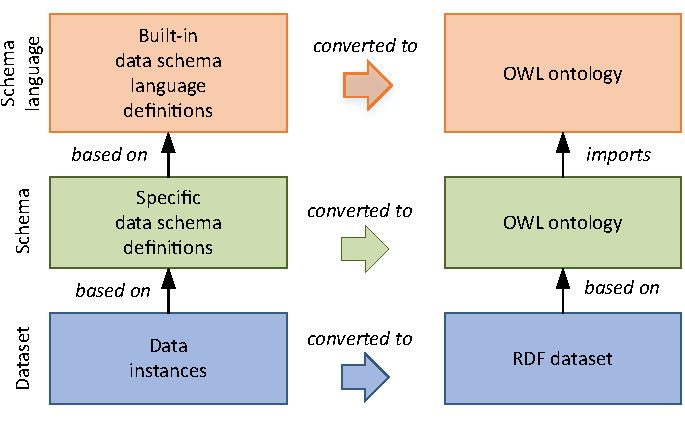
\includegraphics[width=\columnwidth]{images/data-model-components-2.pdf}
    \caption{Conversion of building data model to Web of Data}
    \label{fig:data-model-components}
\end{figure}


However, the research focuses only on the \emph{"pu\-re" sta\-tic mod\-el da\-ta} and ignores the rest part.
"Pure" model data consists of entities, explicit attributes and their values, which (a) represent a product model's state and (b) are needed for data exchange. 
In contrast, derived attributes, functions, procedures, and rules in EXPRESS language are never included in the datasets for data exchange.
Moreover, these elements contain executable statements, which cannot be represented in OWL 2 profiles.
Besides, worksheets, text styles, formulas, and procedures in spreadsheets are also \emph{out} of the question because they are unnecessary for data exchange between computer applications.
Furthermore, this is one of reasons of creating lightweight XML format COBieLite for COBie (Construction Operations Building Information Exchange) data (see \autoref{sec:data-model-classification}).




\subsubsection{Data model classification}\label{sec:data-model-classification}

% Our survey shows that industrial data models specified with the same schema language have many similarities, such as data types, data structures, and object patterns being used within them.
% Therefore, in order to facilitate data model analysis, all data models are divided into three groups, namely (1) EXPRESS-based data models, (2) XSD-based data models, and (3) Tabular and relational data models (see \autoref{tab:data-model-classification}).


The vast majority of data models, used for data exchange in the AEC/FM industry, can be divided into three groups, namely (1) EXPRESS-based data models, (2) XSD-based data models, and (3) Tabular and relational data models (see \autoref{tab:data-model-classification}).
Moreover, the analysis shows that data models, which belong to the same group, often use similar data types, data structures, and object patterns.




\begin{table}\footnotesize
    \centering
    \caption{Data model classification}
    \label{tab:data-model-classification}
    
    \rowcolors{2}{white}{lightgray}
    
    
    \begin{tabulary}{\columnwidth}{p{0.2\columnwidth}p{0.2\columnwidth}p{0.2\columnwidth}p{0.2\columnwidth}}
        \hline
        % \rowcolor{lightgray}
            Data models      &
            EXPRESS-based   &
            XSD-based       &
            Tabular \& \newline relational
        \\
        \hline
            Schema \newline languages &
            EXPRESS & XSD   &
            CSV, \newline Spreadsheet, \newline SQL
        \\
            Data formats &
            STEP-File (SPF),    \newline STEP-XML &
            XML &
            CSV, \newline   Spreadsheet,    \newline RDBMS
        \\            
            Related \newline conceptual \newline models   &
            IFC, \newline COBie &
            IFC, \newline COBie, \newline bsDD, \newline MVD, \newline CityGML, \newline InfraXML, \newline LandXML, \newline internal \newline data \newline formats &
            COBie, \newline internal \newline data \newline formats
        \\
        \hline
    \end{tabulary}
\end{table}






\textbf{1. EX\-PRESS-ba\-sed da\-ta mod\-els} have data schemas specified in EXPRESS language \cite{iso2004express} and their datasets are stored in STEP-File or STEP-XML formats.
EXPRESS is a standard data modeling language for product data that is defined in ISO 10303-11 \cite{iso2004express}, a part of ISO 10303 Product data representation and exchange standard, as known as ISO STEP (Standard for the Exchange of Product model data).
ISO STEP also specifies EXPRESS-G, a graphical notation for a subset of EXPRESS.
An EXPRESS-based data model may have more than one schemas, each of which address a specific subdomain of the domain.
These schemas may be related to each other via schema interfaces.
STEP-File (STEP Physical File, SPF, or STEP) \cite{iso2016stepfile} and STEP-XML \cite{iso2007stepxml} are two data serialization formats, accordingly defined in ISO 10303-21 and ISO 10303-28.




\textbf{2. XSD-\-ba\-sed da\-ta mod\-els} have data schemas specified in XSD (W3C XML Schema Definition) language and their datasets are stored in XML (eXtensible Markup Language) format.
Unlike other schema languages for XML, XSD achieved Recommendation status within the World Wide Web Consortium (W3C) in 2001 .
Its latest version XSD 1.1 \cite{gao2009w3c, peterson2009w3c}, published as a W3C Recommendation in 2012, is especially popular for industrial data models.
Another schema language for XML called RELAX NG (REgular LAnguage for XML Next Generation), an ISO standard, is less popular than XSD and is not analysed here.




\textbf{3. Tabular and relational data models} have data structured in tabular form, i.e. tables with rows and columns.
i.e. sets of rows, where each row cont


While tabular data is stored in files, relational data is stored in relational data base management systems (RDBMS).

Tabular data is exchanged in a variety of formats, such as CSV (comma-separated values) format, tab-delimited format, fixed field format, spreadsheets, HTML tables, and SQL dumps.
CSV (comma-separated values) format is a common data exchange format widely used in scientific applications, however, there are many variants of CSV.
Currently, there are two notable efforts on standardising CSV:
In 2015, W3C published a Recommendation, which defines an abstract tabular data model and specifies so called Best Practice CSV for expressing that tabular data model \cite{tennison2015tabular}.
At the same time, The National Archives (United Kingdom) developed and published the specification of the CSV Schema Language 1.1 \cite{retter2016csv}.  
Spreadsheets are popular among practitioners who use spreadsheet tools, such as Microsoft Excel or Open Office, for analysing data.
There are many spreadsheet formats, for instance, OpenDocument Spreadsheet (.ods), Microsoft Excel (.xlsx), XML Spreadsheet (SpreadsheetML).


Relational data schema is specified with SQL....



Below are short descriptions of data model examples mentioned in \autoref{tab:data-model-classification} and explanations why one conceptual model, such as IFC or COBie, are related to several data model groups in the same time.


\textbf{IFC (Industry Foundation Classes)} is a platform neutral and open product data model, and is the most extensively utilized collaboration data format in BIM.
IFC is developed and published by buildingSMART as openBIM standard IFC (equivalent to ISO 13739:2013) \cite{iso2013ifc}.
Currently, two IFC specifications are officially in use: IFC2x3 TC1 \cite{liebich2007ifc2x3} and IFC4 Add2 \cite{liebich2016ifc4}, because the number of BIM software applications and software vendors granted with IFC4 certification is very little comparing with the ones with IFC2x3 certification.
Each IFC specification include the IFC Product data model (IFC Object model) in several languages: EXPRESS, EXPRESS-G, and XSD \cite{liebich2007ifc2x3, liebich2016ifc4}.
IFC-EXPRESS and IFC-XSD are \emph{almost} equivalent; their distinction is discussed in \autoref{sec:xsd-based-models}.
IFC datasets can be serialised in different file formats, namely IFC-SPF (IFC-STEP), IFC-XML (ifcXML), or IFC-ZIP (ifcZIP).
IFC-SPF datasets are based on STEP-file format and conform to IFC-EXPRESS schema.
Similarly, IFC-XML datasets are based on STEP-XML format and conform to IFC-XSD schema.
IFC-ZIP is a ZIP compressed format consisting of an embedded IFC-SPF.
In addition to the IFC Object model in formal languages, an IFC specification, i.e. an IFC Release documentation, also contain semantic explanations in informal languages, and IFC Property Set definitions (PSDD) in XSD (see details in \ref{sec:xsd-based-models}).


\textbf{COBie (Construction Operations Building Information Exchange)} is an international standard specification of information exchange to capture data during design, construction, and commissioning for handover to facility management \cite{bentley2013cobie, east2007construction}.
COBie, first was published by US Army Corps of Engineer in 2007 and today is jointly maintained by several buildingSMART organizations \cite{day2014problem, karlshoj2016delivering}.
COBie-compliant information can be delivered in four formats: COBie Spreadsheet XML, IFC-SPF, IFC-XML, and COBieLite RC 4 (XML).
COBie Spreadsheet XML, based on SpreadsheetML, is the most common format used by practitioners because it is editable with spreadsheet tools.
IFC-SPF and IFC-XML are used for the delivery of COBie data via IFC, consisting of two steps: (1) the exploration of the native model in IFC format, and (2) the transformation of the IFC model in COBie spreadsheet format \cite{karlshoj2016delivering}. 
As pointed out in \cite{yalcinkaya2015examining}, although "IFC is not all-in-one and the only source for the information requested in COBie specification", it "can be considered as the most convenient source for COBie extraction".
COBieLite is a new NIEM-conformant (National Information Exchange Model) XML format designed to support lightweight COBie information exchanges with Web Services.
Relationships between entities in this format are explicitly defined with XSD and it is free of unnecessary data about spreadsheets, text style and so on \cite{bogen2015cobielite}.
While COBieLite is still under development, the other three formats are officially approved in the British Standard BSI1192-4:2014 about making COBie mandatory for public commissions in UK from April 2016 \cite{karlshoj2016delivering}.




\subsubsection{EXPRESS-based data models}\label{sec:express-based-data-models}

\noindent\textbf{Data schemas}

An EXPRESS-based data model is specified with one or more interrelated schemas.
A schema is a unit or module within the whole EXPRESS model that addresses a specific subdomain of the model and may import another schema of the same model.
A schema consists of different kinds of declarations (see Listing \ref{lst:express-schema-declarations}).
% However, the import and constant declarations are currently unused in the IFC-EXPRESS data schemas.
However, as mentioned in \autoref{sec:scope-of-interest} functions (defined with keyword \texttt{FUNCTION}), procedures (\texttt{PROCEDURE}), global rules (\texttt{RULE}), as well as types constraints (\texttt{WHERE}) and derived attributes (\texttt{DERIVE}) are out of consideration.
Data type declarations (\texttt{TYPE} and \texttt{ENTITY}) \textit{without} constraints and derived attributes are discussed below.

\begin{lstlisting}[caption={The structure of an EXPRESS schema.},label=lst:express-schema-declarations]
SCHEMA IFC4;
  [import declarations]
  [constant declarations]
  [type declarations]
  [function declarations]
  [procedure declarations]
  [rule declarations]
SCHEMA;
\end{lstlisting}




There are six groups of data types in EXPRESS, namely \emph{simple} (\emph{primitive})\footnote{
    To avoid confusion between \emph{EXPRESS simple types}, which are built-in primitive types, and \emph{XSD simple types}, which can be built-in primitive, built-in derived, enumeration, or other types, in this paper EXPRESS simple types are called as \emph{primitive types}.
}, \emph{entity}, \emph{enumeration}, \emph{select}, \emph{aggregation}, and \emph{defined}.

% 
% Simple data types
% 
\emph{Primitive data types} are seven built-in types, including \texttt{IN\-TE\-GER}, \texttt{REAL}, \texttt{NUM\-BER}, \texttt{STRING}, \texttt{BI\-NA\-RY}, \texttt{BOOL\-EAN}, and \texttt{LOG\-I\-CAL}.

EXPRESS \texttt{INTEGER} and \texttt{REAL} values can have in principle any length and accuracy, but most implementations restricted them to signed 32-bit integers
% (equivalent to XSD type \texttt{xs:int})
and floating point doubles.
% (\texttt{xs:double}).
Type \texttt{NUM\-BER} is a super type of \texttt{IN\-TE\-GER} and \texttt{REAL}.

\texttt{STRING} values are finite-length sequences of Unicode (ISO/IEC 10646) characters.
\texttt{BINARY} values are arrays of bits.
Types \texttt{STRING} and \texttt{BINARY} can be specified together with maximum size (see \autoref{lst:express-primitive-types}).
By default, \texttt{STRING} can have any length, \texttt{BINARY} is limited to 32 bit.

\begin{lstlisting}[caption={Examples of \texttt{STRING} and \texttt{BINARY} types with maximum size.},label=lst:express-primitive-types]
TYPE IfcGloballyUniqueId = STRING(22) FIXED;
END_TYPE;

TYPE IfcIdentifier = STRING(255);
END_TYPE;

ENTITY IfcPixelTexture
  ...
  Pixel : LIST [1:?] OF BINARY(32);
END_ENTITY;
\end{lstlisting}



Type \texttt{BOOL\-EAN} with two fixed values \texttt{TRUE} and \texttt{FALSE} is used for traditional Boolean (two-valued) logic.
Type \texttt{LOG\-I\-CAL} has three predefined values: \texttt{TRUE},  \texttt{FALSE}, and \texttt{UNKNOWN}, and it is needed for trivalent (three-valued) logics (3VL).
It is worth mentioning that there many 3VLs \cite{fronthofer2011manyvaluedlogics}, which have different numerical representations for the set of truth values \{\texttt{FALSE}, \texttt{UNKNOWN}, \texttt{TRUE}\}, for instance, \{-1, 0, +1\} (Kleene and Priest logics), \{-1, 0, 0/1\} (redundant binary representation), \{0, 1, 2\} (ternary numeral system), and so on.
In contrast, set \{\texttt{FALSE}, \texttt{TRUE}\} in Boolean algebra is always equivalent to \{0, 1\}.
Therefore, it is not recommended to convert interrelated types \texttt{BOOLEAN} and \texttt{LOGICAL} to number types like in \CPP{} programming language.


\emph{Enumeration data types} represent fixed sets of possible string values.
Different enumeration types may have similar values, for instance, both types \texttt{IfcAddressTypeEnum} and \texttt{IfcColumnTypeEnum} have value \texttt{USERDEFINED} (see \autoref{lst:express-enum-types}).


\begin{lstlisting}[caption={Printout of enumeration types \texttt{IfcAddressTypeEnum} and \texttt{IfcColumnTypeEnum}.},label=lst:express-enum-types]
TYPE IfcAddressTypeEnum = ENUMERATION OF
  ( OFFICE, SITE, HOME, DISTRIBUTIONPOINT, USERDEFINED );
END_TYPE;

TYPE IfcColumnTypeEnum = ENUMERATION OF
  ( COLUMN, PILASTER, USERDEFINED, NOTDEFINED );
END_TYPE;
\end{lstlisting}


\emph{Select data types} are unions of other data types, usually non-primitive ones.
Underlying data types of a select type can be very different to each other.
For instance, select type \texttt{IfcTrimmingSelect} is union of entity type \texttt{IfcCartesianPoint} and defined type \texttt{IfcParameterValue}.



\begin{lstlisting}[caption={Printout of select type \texttt{IfcTrimmingSelect} and its underlying types.},label=lst:express-select-types]
TYPE IfcTrimmingSelect = SELECT
  ( IfcCartesianPoint, IfcParameterValue );
END_TYPE;

ENTITY IfcCartesianPoint
 SUBTYPE OF (IfcPoint);
   Coordinates : LIST [1:3] OF IfcLengthMeasure;
 DERIVE
    Dim: IfcDimensionCount := HIINDEX(Coordinates);
 WHERE
    CP2Dor3D : HIINDEX(Coordinates) >= 2;
END_ENTITY;

TYPE IfcParameterValue = REAL;
END_TYPE;
\end{lstlisting}



\emph{Aggregation data types} are \emph{unnamed} containers of values of exactly \emph{one} other data type
\footnote{In other data models, aggregation data usually consist of values from different types.}.
In other words, they like collection types in Java or C{\#} programming languages.
There are four types of aggregation: \texttt{ARRAY} (ordered, defined with start and end indexes), \texttt{LIST} (ordered, defined with minimum and maximum cardinalities), \texttt{SET} (unordered, all values are unique), and \texttt{BAG} (unordered, no duplicated values).
However, \texttt{BAG} aggregation types are most likely never used in practice.
\texttt{LIST} and \texttt{SET} aggregations can have unlimited maximum cardinality.



\emph{Defined} or \emph{named} data types are used to \emph{name} and add constraints to another data type.
For instance, type \texttt{Ifc\-Length\-Measure} is defined to assign a meaningful name to the simple type \texttt{REAL} (see \autoref{lst:express-defined-types}).
Type \texttt{Ifc\-Positive\-Length\-Measure} is defined to restrict \texttt{Ifc\-Length\-Measure} to be positive and add a corresponding name.
Types \texttt{Ifc\-Complex\-Number} and \texttt{Ifc\-Compound\-Plane\-Angle\-Measure} are defined to identify unnamed aggregation types and also add some constraints.


\begin{lstlisting}[caption={Printout of several defined data types},label=lst:express-defined-types]
TYPE IfcLengthMeasure = REAL;
END_TYPE;

TYPE IfcPositiveLengthMeasure = IfcLengthMeasure;
 WHERE
   WR1 : SELF > 0.;
END_TYPE;

TYPE IfcComplexNumber = ARRAY [1:2] OF REAL;
END_TYPE;

TYPE IfcCompoundPlaneAngleMeasure = LIST [3:4] OF INTEGER;
 WHERE
    MinutesInRange : ABS(SELF[2]) < 60;
    SecondsInRange : ABS(SELF[3]) < 60;
    MicrosecondsInRange : (SIZEOF(SELF) = 3) OR (ABS(SELF[4]) < 1000000);
    ...
END_TYPE;
\end{lstlisting}

% TYPE IfcBoxAlignment = IfcLabel;
%  WHERE
% 	WR1 : SELF IN ['top-left', 'top-middle', 'top-right', 'middle-left', 'center', 'middle-right', 'bottom-left', 'bottom-middle', 'bottom-right'];
% END_TYPE;

% TYPE IfcLabel = STRING(255);
% END_TYPE;


    










    

     

% 
% Entity data types
% 
\emph{Entity data types} are almost similar to classes in traditional object-oriented programming (OOP) languages, with a few exceptions:
(i) they have no operations (methods);
(ii) they have three kinds of attributes: explicit, derived and inverse;
(iii) they contain rules (\texttt{WHERE}-constraints).
\emph{Explicit attributes}, such as \texttt{IfcCompositeCurve.Segments} 

are normal attributes, values of which must be serialised when data exchanging because they characterise their entities.
Explicit attributes of an entity type can have any data type allowed in the data model.
If the value type of an entity type attribute is another entity type then we can say that there is a directed association relationship between two entity types.

The association relationship in the inverse direction is called \emph{inverse relationship}
Assume that entity \texttt{a} of type \texttt{A} has attribute \texttt{x} which has entity type \texttt{B}.
If value of an entity explicit attribute is another entity \texttt{a.x = b}

then we can say that there is an association relationship between them.
\emph{Inverse attributes} 

\emph{Derived attributes} can be derived from other attributes of the same entity using formulas, which contain functions and mathematical operations.

    
    contain derived attributes and type constraints, which are outside the range of consideration, as explained above;
    (iii) they have inverse attributes, which are similar to inverse properties in OWL (see Section ...).
    
    Like classes in Java and C{\#}, an entity data type has \emph{not more than one} super type.
    However, attribute names of subtypes should not duplicate attribute names of their super types.
    Nevertheless, there is no restrictions between attribute names in unrelated classes (it is important).
    Each attribute has a certain data type, which can belong to any of the six data type groups.
    In addition, the order of attribute declarations inside each entity data type is important because it is used for serialisation in the STEP-File format.
    
    
    
\begin{lstlisting}[caption={Examples of EXPRESS entity types},label=lst:express-entity-types]
ENTITY IfcCompositeCurve
 SUPERTYPE OF (ONEOF
    (IfcCompositeCurveOnSurface))
 SUBTYPE OF (IfcBoundedCurve);
	Segments : LIST [1:?] OF IfcCompositeCurveSegment;
	SelfIntersect : IfcLogical;
 DERIVE
	NSegments : IfcInteger := SIZEOF(Segments);
	ClosedCurve : IfcLogical := Segments[NSegments].Transition <> Discontinuous;
 WHERE
	CurveContinuous : ((NOT ClosedCurve) AND (SIZEOF(QUERY(Temp <* Segments | Temp.Transition = Discontinuous)) = 1))  = 0));
	SameDim : SIZEOF( QUERY( Temp <* Segments | Temp.Dim <> Segments[1].Dim)) = 0;
END_ENTITY;

ENTITY IfcCompositeCurveSegment
 SUPERTYPE OF (ONEOF
    (IfcReparametrisedCompositeCurveSegment))
 SUBTYPE OF (IfcGeometricRepresentationItem);
	Transition : IfcTransitionCode;
	SameSense : IfcBoolean;
	ParentCurve : IfcCurve;
 DERIVE
	Dim : IfcDimensionCount := ParentCurve.Dim;
 INVERSE
	UsingCurves : SET [1:?] OF IfcCompositeCurve FOR Segments;
 WHERE
	ParentIsBoundedCurve : ('IFC4.IFCBOUNDEDCURVE' IN TYPEOF(ParentCurve));
END_ENTITY;
\end{lstlisting}    
    
    
    
    
    
    
% ENTITY IfcContext
%  ABSTRACT SUPERTYPE OF (ONEOF
%     (IfcProject
%     ,IfcProjectLibrary))
%  SUBTYPE OF (IfcObjectDefinition);
% 	ObjectType : OPTIONAL IfcLabel;
% 	LongName : OPTIONAL IfcLabel;
% 	Phase : OPTIONAL IfcLabel;
% 	RepresentationContexts : OPTIONAL SET [1:?] OF IfcRepresentationContext;
% 	UnitsInContext : OPTIONAL IfcUnitAssignment;
%  INVERSE
% 	IsDefinedBy : SET [0:?] OF IfcRelDefinesByProperties FOR RelatedObjects;
% 	Declares : SET [0:?] OF IfcRelDeclares FOR RelatingContext;
% END_ENTITY;


% ENTITY IfcObject
%  ABSTRACT SUPERTYPE OF (ONEOF
%     (IfcActor
%     ,IfcControl
%     ,IfcGroup
%     ,IfcProcess
%     ,IfcProduct
%     ,IfcResource))
%  SUBTYPE OF (IfcObjectDefinition);
% 	ObjectType : OPTIONAL IfcLabel;
%  INVERSE
% 	IsDeclaredBy : SET [0:1] OF IfcRelDefinesByObject FOR RelatedObjects;
% 	Declares : SET [0:?] OF IfcRelDefinesByObject FOR RelatingObject;
% 	IsTypedBy : SET [0:1] OF IfcRelDefinesByType FOR RelatedObjects;
% 	IsDefinedBy : SET [0:?] OF IfcRelDefinesByProperties FOR RelatedObjects;
%  WHERE
% 	UniquePropertySetNames : ((SIZEOF(IsDefinedBy) = 0) OR IfcUniqueDefinitionNames(IsDefinedBy));
% END_ENTITY;

    
    

    

    
    % Each defined data type can be considered as a named subset (or an equivalent set) of another data type.
    % Without going into detail of type constraints, we can say the following things about the defined data types in \ref{lst:express-defined-types}:
    % \texttt{IfcPositiveLengthMeasure} \subseteq \texttt{IfcLengthMeasure} \equiv \texttt{REAL}
    
    
    % Consider the sample types in Listing \ref{lst:express-defined-types}.
    % The defined type \texttt{IfcPositiveLengthMeasure} is a subset of another defined type \texttt{IfcLengthMeasure}, which in turn is equal to the simple type \texttt{REAL}.
    % The defined type \texttt{IfcBoxAlignment} is a subset of another defined type \texttt{IfcLabel}, which represents a subset \texttt{STRING}








% % According to the mapping methodology from IFC-EXPRESS to IFC-XSD, simple data types \texttt{STRING}, \texttt{INTEGER}, \texttt{REAL}, \texttt{NUMBER}, \texttt{BOOLEAN} are mapped to equivalent standard \texttt{XSD} types, namely \texttt{xs:string} (sometimes \texttt{xs:nor\-ma\-li\-zed\-String}), \texttt{xs:in\-te\-ger}, \texttt{xs:dou\-ble} (twice), and \texttt{xs:\-boo\-le\-an}.
% % In the same time simple data types \texttt{LOGICAL} and \texttt{BINARY} are translated into user defined types \texttt{ifc:lo\-gi\-cal} and \texttt{ifc:hex\-Bi\-na\-ry}.


% In the IFC-EXPRESS schema, all data types for calendar and duration values are defined types, not included in EXPRESS (Listing \ref{lst:express-calendar-types}).

% \begin{lstlisting}[caption={Examples of calendar-related data types},label=lst:express-calendar-types]
% TYPE IfcTime = STRING;
% END_TYPE;

% TYPE IfcTimeMeasure = REAL;
% END_TYPE;

% TYPE IfcTimeStamp = INTEGER;
% END_TYPE;


% TYPE IfcDate = STRING;
% END_TYPE;

% TYPE IfcDateTime = STRING;
% END_TYPE;

% TYPE IfcDuration = STRING;
% END_TYPE;



% \end{lstlisting}


% TODO: Add some example of an entity data type


% % <xs:simpleType name="IfcLogical">
% % 		<xs:restriction base="ifc:logical"/>
% % 	</xs:simpleType>
	
% % 	<xs:simpleType name="IfcMassFlowRateMeasure">
% % 		<xs:restriction base="xs:double"/>
% % 	</xs:simpleType>
	
	
% % 	<xs:simpleType name="IfcTime">
% % 		<xs:restriction base="xs:normalizedString"/>
% % 	</xs:simpleType>
% % 	<xs:simpleType name="IfcTimeMeasure">
% % 		<xs:restriction base="xs:double"/>
% % 	</xs:simpleType>
% % 	<xs:simpleType name="IfcTimeStamp">
% % 		<xs:restriction base="xs:long"/>
% % 	</xs:simpleType>
	
	
% % 		<xs:simpleType name="IfcDate">
% % 		<xs:restriction base="xs:normalizedString"/>
% % 	</xs:simpleType>
% % 	<xs:simpleType name="IfcDateTime">
% % 		<xs:restriction base="xs:normalizedString"/>
% % 	</xs:simpleType>











% % EXPRESS defines 


% % According to terminology of EXPRESS, 

% % , which are a bit different to the data models used traditional OOP (object-oriented programming) languages.
% % In particular, an attribute in EXPRESS may have multiple values, similarly to properties in OWL and unlike class attributes in traditional OOP.
% % Another difference is that lists and sets in EXPRESS may have both minimum and maximum cardinalities, again similarly to OWL.
% % ...
% % Tabular and relational data models are related with such terms as tables, rows and columns.
% % And for that reason, spreadsheets also belong to this category.



% % \begin{table}[!th]
% %     \centering
% %     \begin{tabular}{c|c|c|c}
% %         \hline
% %         Group & EXPRESS-bases & XSD-based & Tabular \& relational data \\
% %         \hline
% %         Data schema & IFC-EXPRESS & IFC-XSD & \\
% %         \hline
% %     \end{tabular}
% %     \caption{Caption}
% %     \label{tab:my_label}
% % \end{table}










% % Firstly, 

% % , such as 




% % The SPF-based formats are the data formats 








% % , which, however, have similar properties.
% % They are: SPF, 





% \input{part-212-xsd-based-models.tex}

% \input{part-22-linked-building-data.tex}


% \input{part-23-current-data-mapping.tex}
% \input{part-231-express-to-xsd.tex}
% \input{part-232-express-to-ld.tex}
% \input{part-233-.tex}


% \newpage



% \section{Methodology}


% \subsection{Data model comparison}\label{sec:data-model-comparison}

All data models discussed in \autoref{sec:state-of-the-art} are driven not only by schema languages features, but also by related common practices.
\autoref{tab:data-model-comparison} shows which main features are used in EXPRESS-driven and XSD-driven building data models, and how they are supported by OWL 2 profiles.

% \blindtext
% \thispagestyle{empty}
% \begin{landscape}




\begin{table*}[t]
% \begin{sidewaystable}[t]
\footnotesize
    \centering
    \caption{Data model comparison}
    \label{tab:data-model-comparison}
    
    % \rowcolors{4}{lightgray}{}    

    \begin{threeparttable}    
        \begin{tabu} to \textwidth { X[0.5] X[0.6l] X[l] X[l] X[l] X[l] X[l] }            
            \hline            
                \multirow{2}{*}{\textbf{Features}}
                & \multicolumn{2}{c|}{\textbf{Used in building data models}}
                & \multicolumn{4}{c}{\textbf{Supported by OWL 2 profiles}}
            \\    
            \cline{2-7}            
                & \multicolumn{1}{l}{\textbf{EXPRESS-}}
                & \multirow{2}{*}{\textbf{XSD-driven}}
                & \multirow{2}{*}{\textbf{OWL 2 EL}}
                & \multirow{2}{*}{\textbf{OWL 2 QL}}
                & \multirow{2}{*}{\textbf{OWL 2 RL}}
                & \multirow{2}{*}{\textbf{OWL 2 DL}}
            \\    
                & \textbf{driven}    
                &
                &
                &
                &
                &
            \\    
            \hline            
            \hline
                \multicolumn{7}{c}{\textbf{Primitive Types}}
            \\
            % \hline            
                Decimals  % Feature  
                
                & \texttt{REAL}       % EXPRESS
                
                & \texttt{\textit{xs:decimal\tnotex{tn:rarely-used}}  \newline xs:double}      % XSD
                
                & \texttt{owl:real    \newline    owl:relational  \newline xsd:decimal}     % EL
                
                & \texttt{xsd:decimal \newline xsd:double}     % QL
                
                & \texttt{xsd:decimal \newline xsd:double}     % RL
            
                & \texttt{owl:real \newline owl:relational    \newline xsd:decimal \newline xsd:double}     % RL
            \\
            % \hline            
                Integers    % Feature
                
                & \texttt{INTEGER}       % EXPRESS
                
                & \texttt{\textit{xs:int\tnotex{tn:rarely-used}} \newline xs:integer \newline xs:long \newline
                \textit{xs:nonNegInt\tnotex{tn:xsd-nonNegInt}\tnotex{tn:rarely-used}}}  % XSD
                
                & \texttt{xsd:integer \newline xsd:nonNegInt\tnotex{tn:xsd-nonNegInt}}  % EL
                
                & \texttt{xsd:integer \newline xsd:nonNegInt\tnotex{tn:xsd-nonNegInt}}  % QL
                
                % & \texttt{xsd:int \newline xsd:integer \newline xsd:long \newline xsd:non\newline-Negative\newline-Integer}  % RL
                & \texttt{xsd:int \newline xsd:integer \newline xsd:long \newline xsd:nonNegInt\tnotex{tn:xsd-nonNegInt}}  % RL
                
                & \texttt{xsd:int \newline xsd:integer \newline xsd:long \newline xsd:nonNegInt\tnotex{tn:xsd-nonNegInt}}  % DL
            \\
            % \hline            
                Strings    % Feature
                
                & \texttt{STRING}       % EXPRESS
                
                & \texttt{\textit{xs:ID\tnotex{tn:rarely-used}  \newline xs:language\tnotex{tn:rarely-used}  \newline xs:NMTOKENS\tnotex{tn:rarely-used}}\newline
                xs:normString\tnotex{tn:normString}  \newline    xs:string}      % XSD
                
                & \texttt{xsd:normString\tnotex{tn:normString}   \newline xsd:string}    % EL
                
                & \texttt{xsd:normString\tnotex{tn:normString}   \newline xsd:string}     % QL
                
                & \texttt{xsd:normString\tnotex{tn:normString}   \newline xsd:string}     % RL
                
                & \texttt{xsd:normString\tnotex{tn:normString}   \newline xsd:string}     % DL
            \\
            % \hline            
                Booleans    % Feature
                
                & \texttt{BOOLEAN}       % EXPRESS
                
                & \texttt{xs:boolean}      % XSD
                
                & --\tnotex{no-built-in-support}    % EL
                
                & --\tnotex{no-built-in-support}     % QL
                
                & --\tnotex{no-built-in-support}     % RL
                
                & \texttt{xs:boolean}      % DL
            \\
            % \hline            
                Logicals    % Feature
                
                & \texttt{LOGICAL}       % EXPRESS
                
                & as enumeration      % XSD
                
                & --\tnotex{no-built-in-support}    % EL
                
                & --\tnotex{no-built-in-support}     % QL
                
                & --\tnotex{no-built-in-support}     % RL
                
                & --\tnotex{no-built-in-support}      % DL
            \\
            % \hline            
                Time \newline instances    % Feature
                
                & --\tnotex{no-built-in-support}       % EXPRESS
                
                & \texttt{xs:date \newline xs:dateTime \newline xs:time \newline xs:gYear}      % XSD
                
                & --\tnotex{no-built-in-support}    % EL
                
                & --\tnotex{no-built-in-support}     % QL
                
                & --\tnotex{no-built-in-support}     % RL
                
                & --\tnotex{no-built-in-support}      % DL
            \\
            % \hline            
                Names \& IDs    % Feature
                
                & --\tnotex{no-built-in-support}       % EXPRESS
                
                & \texttt{xs:anyURI \newline xs:IDREF \newline xs:QName}      % XSD
                
                & \texttt{xs:anyURI}    % EL
                
                & \texttt{xs:anyURI}     % QL
                
                & \texttt{xs:anyURI}     % RL
                
                & \texttt{xs:anyURI}      % DL
            \\
            \hline
        \end{tabu}
        \begin{tablenotes}
        %   \item\label{tn:xs-prefix} Types with prefixes \textit{xs:}
          \item\label{tn:rarely-used} Rarely used.
          \item\label{tn:a} Element declarations
          \item\label{tn:xsd-nonNegInt} \texttt{nonNegativeInteger}
          \item\label{tn:normString} \texttt{normalizedString}
          \item\label{tn:logical} Three-value logical values
          \item\label{no-built-in-support} No built-in support, requires special solutions
        \end{tablenotes}
    \end{threeparttable}    
\end{table*}
% \end{sidewaystable}

% \end{landscape}





% \subsection{Target criteria}

% \textbf{Requirement to input data models}
% ...


% \textbf{Requirement to output data formats}
% ...

% \textbf{Conversion schema}




% \subsection{Data models comparison}





% % The analysis of the simple and well-defined data models, used in the AEC/FM industry and described in Section \ref{sec:state-of-the-art}, shows that in spite of their different nature, they have a lot of similarities.

% In this subsection, the \emph{"pure"} data part of the \emph{simple} and \emph{well-defined} data models, used in the \emph{AEC/FM industry} and described in Section \ref{sec:state-of-the-art}, are compared to each other.
% "Pure" data means the static and most important information content needed for data exchange in the industry.
% Examples of "dirty" data are: worksheets and text styles in spreadsheet formats, derived attributes, functions and rules in the EXPRESS data schemas.
% "Simple" data models do not contain complex elements, such as \texttt{mixed} elements in XSD (see subsection \ref{sec:xsd-based-data-models}), \texttt{BAG}-aggregation data types in EXPRESS (see subsection \ref{sec:express-based-data-models}) or \texttt{image} in relational databases.
% "Well-defined" data models are designed by qualified researchers and engineers, using the latest computer science trends and data modeling best practices.
% The data models used outside the industry are unpredictable, for instance, their entities may not contain unique keys for linking.
% Therefore, data models, which are complicated, or "poorly" designed, or unused in the industry, are outside the scope of the research.
% In general, all the mentioned restrictions help to ensure that the data models are \emph{predictable} and probably can be mapped to the dynamic data model, specified in Section 3.2.





% In spite of different nature of the EXPRESS-based, the XSD-based, and the relational data models groups, these data models have two significant similarities:

% \begin{enumerate}

% \item
% These data models can be mapped in a certain way to an \emph{object} model. All EXPRESS-based data models are object models by definition. Most of XSD schemas are designed on top of a conceptual model, which involves two basic relationships between different "concepts": \emph{inheritance} and \emph{association}.
% The whole-part relationships (aggregations in UML), often used in XSD/XML, are special cases of associations.
% These "concepts" are reflected in certain XSD elements and can be "restored" from the XSD to be classes.
% In tabular or relational data, each table can be considered as a class, which has associations with other classes.

% \item
% Most of \emph{single data records} in datasets of these data models can be considered as entity instances.
% Examples of single data records are: single lines in SPF, rows in tabular and relational data, or XSD-elements in XML.
% However, 


% \item
% All primitive data types used in the data models are related to the following groups: strings, integers, decimals, logicals, binaries, and date-times.


% Entity types are similar to classes in OOP.
% Rows in SPF, CSV, spreadsheets and relational databases, or XSD-elements in XML are samples of single data records. 
% Rows in SPF are instances of entity types by definition.
% \end{enumerate}
% First, \emph{most} (not all) of 
% In case of tabular and relational data models, the table names can be used to define entity types.
% Second, these classes have attributes, but no operations.
% Like in EXPRESS or OWL, and unlike traditional OOP, each attribute may have multiple value.




% Third, there are only two basic relationships between these classes, namely inheritance and association.
% Each class has only one superclass. 


% ... In the Sections ..., we analyse in details each group of data models, which parts of them can or cannot be converted into OWL and RDF.


% % (4) each attribute 

% % The main difference between such a class diagram and an object model in traditional object-oriented programming (OOP) languages is that it allows attributes to have multiple values, similarly to properties in OWL languages (see...).



% % Firstly, all simple data types are related to one of the following groups: strings, integers, decimals, enumerations, calendar, and logical. 




% % The specific features of the data schemas to be ignored, for instance, are: functions, derived attributes and rules in EXPRESS; ... in XSD; data about workbooks, worksheets, text style and so on in Spreadsheets.










% Remember: Meta data (about whole dataset) and annotations (about each elements)




% \subsection{IFC-EXPRESS-to-OWL and IFC-SPF-to-RDF conversion}


% \subsection{Target criteria}


% \subsection{Building Entity Abstract Model}

% (Several class diagrams)

% (BEAM or BEM?)



% \subsection{BEAM-to-LD conversion principles}

% Summaring principles for each data types and properties


% \newpage



% \section{BEAM-to-LD converter}

% \subsection{Architecture and key features}


% 1. Why not straightforward conversion


% 2. Common conversion schema

% 2. 




% \subsection{Experimental results}

% Comparison with previous implementations

% OWL conformance validation, ...

% \newpage


% \section{Discussion}


% \section{Summary}

% \section{Acknowledgement}

%%%%%%%%%%% The article body starts:

%\section{}\label{s1}

%\subsection{}\label{s1.1}






%\begin{figure}[t]
%\includegraphics{}
%\caption{Figure caption.}\label{f1}
%\end{figure}

%\begin{table*}
%\caption{} \label{t1}
%\begin{tabular}{lll}
%\hline
%&&\\
%&&\\
%\hline
%\end{tabular}
%\end{table*}


%%%%%%%%%%% The bibliography starts:
% \begin{thebibliography}{9}

\bibliographystyle{plain}
\bibliography{part-99-bibliography}


% \bibitem{r1}
% \bibitem{r2}

% \end{thebibliography}



\end{document}
